% \documentclass{article}

% % Language setting
% % Replace `english' with e.g. `spanish' to change the document language
% \usepackage[english, russian]{babel}

% % Set page size and margins
% % Replace `letterpaper' with `a4paper' for UK/EU standard size
% \usepackage[letterpaper,top=2cm,bottom=2cm,left=3cm,right=3cm,marginparwidth=1.75cm]{geometry}

% % Useful packages
% \usepackage{amsmath}
% \usepackage{color}
% \usepackage{xcolor}
% \usepackage[dvipsnames]{xcolor}
% \usepackage{graphicx}
% \usepackage[colorlinks=true, allcolors=blue]{hyperref}
% \usepackage{color}   %May be necessary if you want to color links
% \usepackage{hyperref}
% \hypersetup{
%     colorlinks=true, %set true if you want colored links
%     linktoc=all,     %set to all if you want both sections and subsections linked
%     linkcolor=blue,  %choose some color if you want links to stand out
% }
\documentclass{article}

% Language setting
% Replace `english' with e.g. `spanish' to change the document language
\usepackage[english, russian]{babel}
\usepackage{amsmath}

%графика
\usepackage{wrapfig}
\usepackage{graphicx}
\usepackage{pgfplots}
\usepackage{tikz}


\usepackage{tcolorbox}

% Set page size and margins
% Replace `letterpaper' with `a4paper' for UK/EU standard size
\usepackage[letterpaper,top=2cm,bottom=2cm,left=3cm,right=3cm,marginparwidth=1.75cm]{geometry}

% Useful packages
\usepackage{amsmath}
\usepackage{amssymb}
\usepackage{graphicx}
\usepackage{fixltx2e}
\usepackage[colorlinks=true, allcolors=blue]{hyperref}

\usepackage{geometry}
\geometry{left=25mm,right=25mm,
 top=25mm,bottom=25mm}

\title{EQUITY VALUATION CONCEPTS AND BASIC TOOLS}
\author{Bidva Maxim}
% Колонтитулы
\usepackage{fancyhdr}
\pagestyle{fancy}
\renewcommand{\headrulewidth}{0.1mm}  
\renewcommand{\footrulewidth}{0.1mm}
\lfoot{}
\rfoot{\thepage}
\cfoot{}
\rhead{CMF-2022}
\chead{}




\begin{document}
\maketitle
\tableofcontents
\newpage
\section{Что такое переоценённые и недооценённые акции}
% Difference between intrinsic (fundamental) value and market value is the source of profits.
% Securities that are followed by many investors are more likely to be fairly valued
В теории существует фундаментальная стоимость (то есть та стоимость которую
был бы готов уплатить рациональный инвестор который обладает абсолютно полной информацией о компании).\\
Чем большее количество инвесторов следит за бумагой, тем ближе текущая рыночная стоимость к вот такой фундаментальной обоснованной оценке.\\
Если находить какие-то акции, где рынок гораздо менее эффективный, то можно зарабатывать дополнительную доходность.\\
Акция на рынке стоит  дешевле, чем её фундаментальная стоимость, значит она недооценена(undervalued), если выше, чем фундаментальная оценка - переоценена(overvalued)

\section{Три группы подходов к оценке акций}
\begin{itemize}
    \item Модели приведённой стоимости(Present value models)\\
(привеённой, потому что в ходе анализа мы приводим будущие денежные потоки к настоящему моменту)
 эта группа методов в своей основе имеет постулат о том, что справедливая фундаментальная стоимость должно быть равна сумме всех будущих денежных потоков, которые инвестор мог бы получить проинвестировав в эту ценную бумагу.
  Так как существует временная стоимость денег, то будущие денежные потоки нужно дисконтировать и приводить их к настоящему моменту.
  \begin{itemize}
    \item dividend models
    \item free-cash-flow-to-equity models
  \end{itemize}
\item Модели мультипликаторов(Multiplier models)
Имеет дело с относительной оценкой. Считаем, что получить точную фундаментальную сложно, поэтому эффективнее будет сравнить акции между собой.
\begin{itemize}
 \item price multiples
 \item enterprise value multiplies
\end{itemize}
\item Модели основанные на оценке активов (Asset-based models)
Мы знаем из бухгалтерского баланса, что стоимость капитала равна разнице между стоимости активов и стоимости обязательств. Таким образом если произвести точную оценку чистых активов, то можно получить и более точную оценку капитала и соответственно стоимости самих активов.
\end{itemize}
\section{Дивиденды}
{\bf Дивиденды(Dividends)} - выплата, которую компания осуществляет в пользу своих акционеров.\\
{\bf Регулярные дивиденды (Regular Cash)} прописаны в уставе компании и выплачиваются регулярно.\\
{\bf Специальные дивиденды(Extra/Special dividends)} выплачиваются если происходит какое-то единоразовое событие.\\
{\bf Stock dividends} - дивиденды, выплакивающиеся в акциях.\\
{\bf Stock split} - увеличение количества акций в обращении но при этом уменьшение номинальной стоимости каждой акции.\\
{\bf Reverse Stock Split} - уменьшение количества акций в обращении, но увеличение номинальной цены каждой акции.\\
(например если у компании очень долгое время бал негативные тренды и акции начинают стоит совсем дешево)\\
{\bf Обратный выкуп акций (Share Repurchases / buybacks)} - процедура, когда компания выкупает акции обращающиеся на бирже на открытом рынке на собственные баланс и затем погашает их, то есть таким образом в свободном обращении становится гораздо меньше акций.\\
\begin{center}
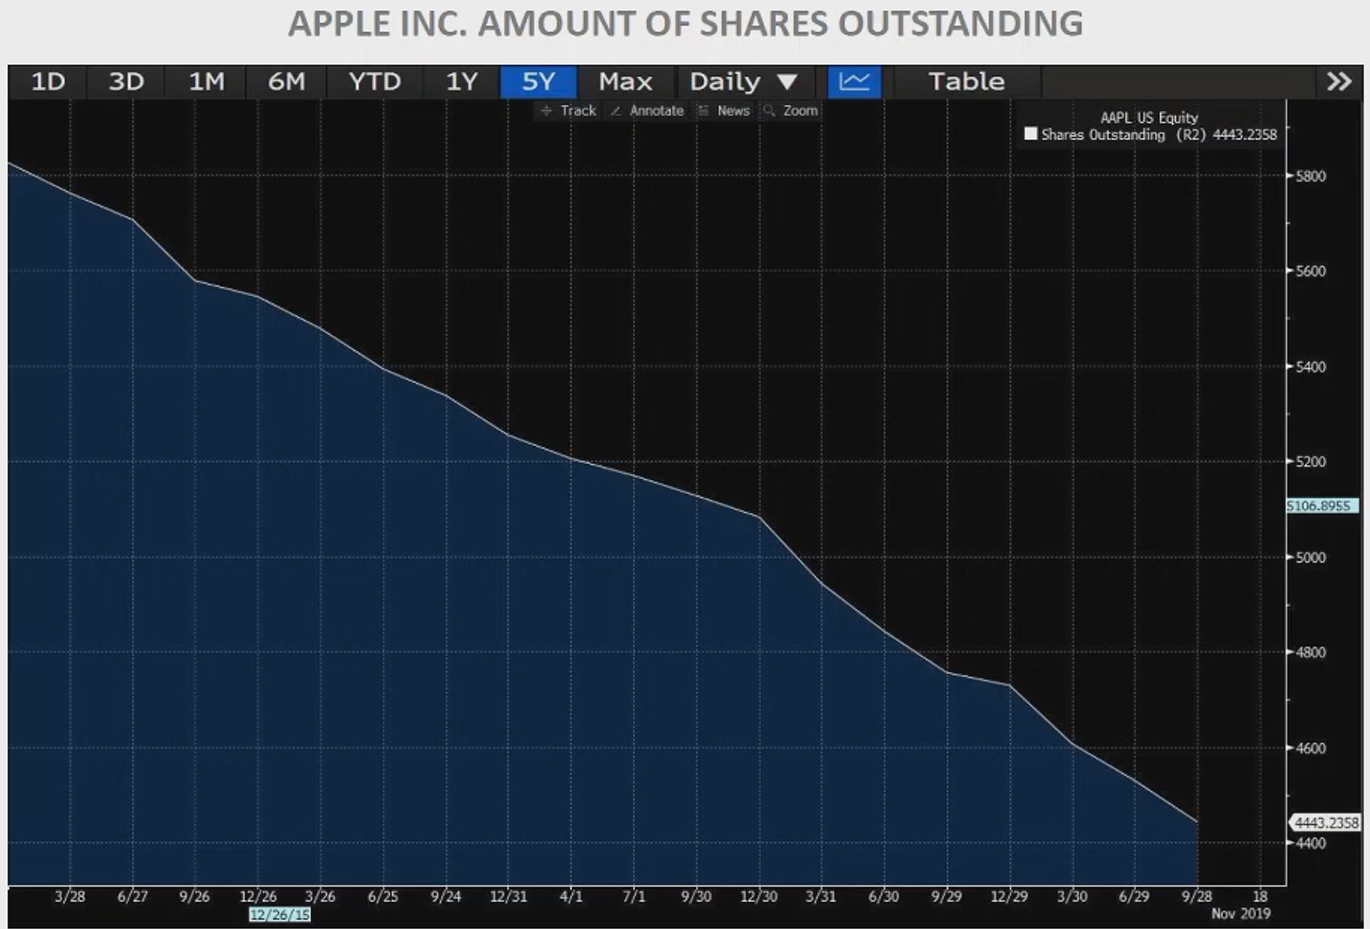
\includegraphics[width=0.75\textwidth]{Apple.png}\\
{Количество акций Apple в обращении за последние 5 лет}
\end{center}
{\bf Declaration date} - дата объявления дивидендов\\
{\bf Ex. date} - дата, когда акция торгуется без дивидендов\\
{\bf Дата отсечки (Record date)} - дата, когда компания проверяет риестор акционеров и определяет кто именно будет получать дивиденды.\\
{\bf Дата выплаты (Payment date)} - день, когда происходит перечисление денег на счёт инвесторов\\
\begin{center}
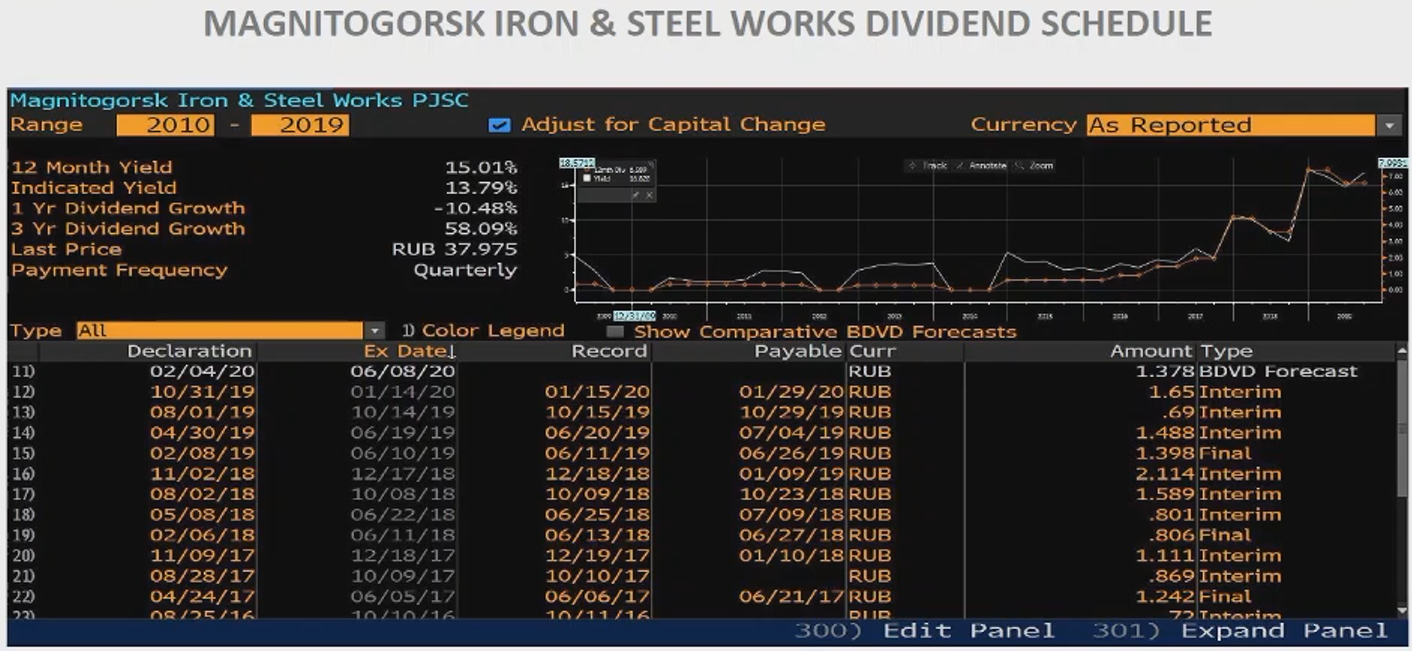
\includegraphics[width=0.75\textwidth]{Magnitagorsz.png}\\
{Последние дивиденды магнитогорского металлургического комбината}
\end{center}

\begin{center}
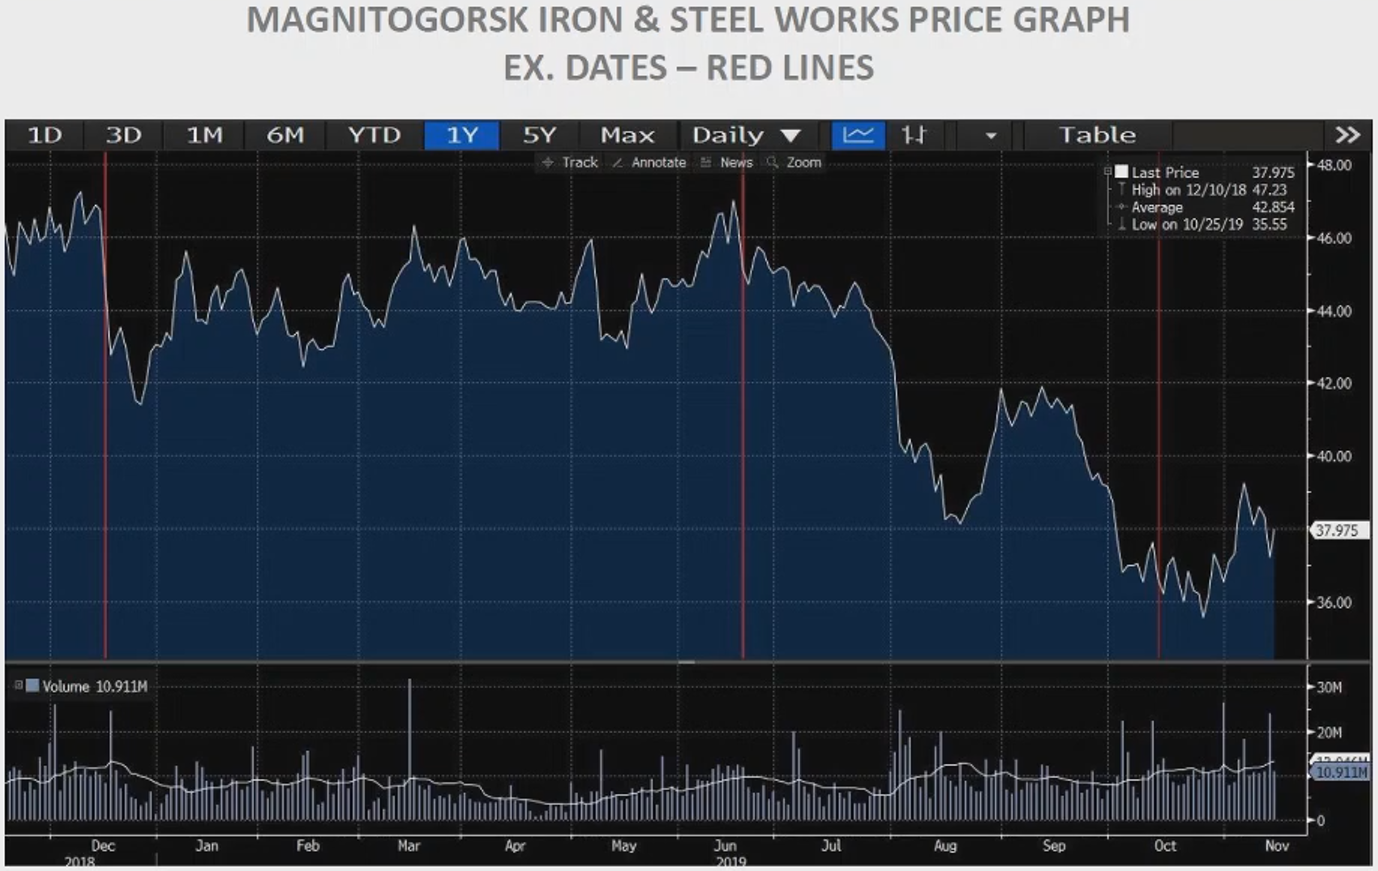
\includegraphics[width=0.75\textwidth]{EX_date.png}\\
{График акций магнитогорского металлургического комбината(красным отмечены EX date)}
\end{center}
\\В даты ex. date акция падает. Так происходит, потому что многим инвесторам которые хотят продать акцию выгодно это сделать в ex date.

\section{Модель дисконтированных дивидендов(DDM)}
Вся группа моделей приведенной стоимости отталкивается от идеи в том, что фундаментальная стоимость внутренняя стоимость должна быть эквивалентна приведенной стоимости всех будущих денежных потоков.\\
Самый типичный денежный поток, который получают акционеры - дивиденды, поэтому логично будет взять и подставить будущий поток дивидендов в нашу модель.\\
$V_0 = \sum_{t=1}^{\infity}\frac{D_t}{(1+k_e)^t}$\\
$V_0$ - фундаментальная стоимость\\
$D_t$ - дивиденды во время t\\
$K_e$ - требуемая ставка доходности при инвестировании в бумагу(required rate of return on common equity)\\
\\
Самый простой тип такой модели - DDM при инвестировании на 1 год.\\
Усложнение - инвестор держит бумагу несколько лет, нужно посчитать приведённую стоимость дивидендов на несколько лет вперёд и прибавить к этому
ожидаемую стоимость(так же известную как terminal value) по которой инвестор закроет свою позицию\\
Пример: Инвестор вкладывает деньги на 2 года, компания платит дивиденды в размере 5 долларов первый год, 6 долларов во второй год после этого инвестора ожидает продать бумагу за 110 \$. Требуется посчитать справедливую стоимость такой бумаги, если требуемая ставка доходности 10 \% 
$V_0 = \frac{5}{(1 + 0.1)^1} + \frac{6}{(1 + 0.1)^2} + \frac{110}{(1 + 0.1)^2} = 100,4$\\
(Продисконтировали дивиденды и сложили)
\section{Free-cash-flow-to-equity модели}
Многие компании не платят дивиденды. В таких случаях используют модели Free-cash-flow-to-equity.\\
FCFE - объем денежных средств которые причитаются именно акционером компании.\\
FCFE = Чистая прибыль + обесценивание - увеличение оборотного капитала - инвестиции в основной капитал -  погашение основного долга + новые долговые обязательства\\
FCFE = объём денежных средств от повседневной деятельности - проведённые инвестиции + займы\\

\section{Оценка привилегированных акций}

Пусть компания по уставу выплачивает каждый год в виде дивидендов по привилегированной акции одну и ту же величину $D_p$.\\
Считаем цену привилегированной акции:\\
Preferred stock value = $\frac{D_p}{(1+k_p)^1} + \frac{D_p}{(1+k_p)^2} + ... + \frac{D_p}{(1+k_p)^x} = \frac{D_p}{k_p}$\\
Пример: Есть компания которая платит 7 \$ на акцию одну привилегированную акцию. Как рассчитать внутреннюю стоимость такой акции, если требуемая ставка доходность составляет 15 \% ?.\\
$V_0 = \frac{7}{15\%} = 46,67$USD\\

\section{Модель роста Гордона}
Считаем, что размер дивиденда растёт фиксированным темпом роста.\\ 
$V_0 = \frac{D_0 (1 + g_c)}{(1 + k_e)^1} + \frac{D_0 (1 + g_c)^2}{(1 + k_e)^2} + ... + \frac{D_0 (1 + g_c)^{\infty}}{(1 + k_e)^{\infty}}$\\
$V_0 = \frac{D_0 (1+g_c)}{k_e - g_c} = \frac{D_1}{k_e - g_c}$\\
$V_0$ - приведенная стоимость\\
$D_0$ - дивиденд в нулевой период\\
$g_c$ - годовой темп роста дивидендов\\
$K_e$ - требуемая доходность\\
Пример: Компания только что заплатила годовой дивиденд в размере 10 \$, ожидаемый темп роста
дивидендов равен 5 \%, ставка дисконтирования равна 15 \%.  Найдите величину ожидаемого дивиденда.\\
$V_G = \frac{10*(1+5\%)}{15\% - 5\%} = \frac{10,5}{0,1} = 105$ USD\\
Какая часть оценочной стоимости акций обусловлена ростом дивидендов?\\
1) Считаем ответ при g = 0\\
2) Вычитаем это значение из оценке без обнуления g.\\
$V_0 = \frac{10}{15\%} = 66,7$USD - если бы не наращивала дивиденды\\
Difference =  105 - 66,7 = 38,3 USD насколко рост дивидендов увеличивает стоимость акции
\section{Как установить ожидаемый темп роста дивидендов.}
\begin{itemize}
    \item Исторический темп роста(например если компания в несколько десятилетий со средним  темпом x\% увеличивала дивиденды, то можно сделать допущение, что в будущем она тоже будет увеличивать дивиденды на x\%) 
    \item Взять медианный показатель по индустрии
    \item Оценка устойчивого темпа роста 
\end{itemize}
  Устойчивый рост(Sustainable growth) - такой темп при котором компания может одновременно и финансировать свои собственные проекты и выплачивать дивиденды.\\

Retention rate = 1 - divident payout ration
dpr - величина, которая показывает какую часть чистой прибыли компания направляет на дивиденды.\\
Sustainable growth rate 

Величина устойчивого темпа роста(Sustainable growth rate) = retention rate * ROE, где ROE(return on equity) это балансовая доходность акций на то что компания зарабатывает на капитал.
\newpage
\section{Модель с несколькими этапами роста(Multistage DDM)}
Считаем, что компания на первом этапе быстро растут, а затем темп роста становится более низким.\\
value = $\frac{D_1}{(1+k_e)^1} + \frac{D_2}{(1+k_e)^2} + ... + \frac{D_n}{(1+k_e)^n} + \frac{P_n}{(1+k_e)^n}$\\
$P_n = \frac{D_{n + 1}}{k_e - gc}$\\
Шаги:
\begin{itemize}
    \item Определить k
    \item Определить на протяжении скольких периодов и с каким темпом g* растут дивиденды
    \item Определить величины девидендов в начальные периоды
    \item Определить скорость роста $g_c$ на втором этапе
    \item Определить $D_n$ первый дивиденд на втором этапе
    \item Посчитать стоимость акций в конце периода быстрого роста
    \item Прибавить pv всех дивидендов к pv $P_n$ 
\end{itemize}

Пример: Аналитик используют такую модель Multistage DDM известно что в прошлом году компания заплатила 2 \$ дивидендов. Инвестор ожидает, что дивиденды будут расти и 15 \% в течение следующих трех лет а после этого темп роста вернется к нормальному и стал ставят 7 \%. Используется ставка дисконтирования 12 \%. Какова справедливая стоимость таких акций?\\
\begin{center}
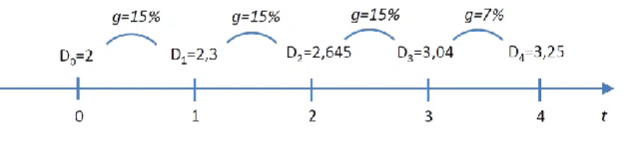
\includegraphics[width=0.75\textwidth]{multistage_ddm.png}\\
\end{center}
1)$k_e$ = 12\%, $g_c$ = 7\%, $D_4$ = 3,25\\
2)$P_3 = \frac{D_4}{k_e - g_c} = \frac{3,25}{15\% - 7\%} = 65,08$\\
3)value = $\frac{2,3}{(1+12\%)^1} + \frac{2,645}{(1+12\%)^2} + \frac{3,04}{(1+12\%)^3} + \frac{65,08}{(1+12\%)^4} = 52,6$\\
\section{Какую модель мы используем в зависимости от рода компании}
Для стабильных компаний которые находятся на уже конечных стадиях жизненного цикла и у них не ожидается резких скачков можно использовать модель гордона.\\
\\
Если же мы имеем дело с компаниями которые находятся на более ранних стадиях жизненного цикла которые испытывают бога высокие темпы роста тогда можно использовать модели мальте стейдж в которых на первом этапе дивиденды растут с высоким темпам роста а на втором этапе они успокаиваются и применяются формулы гордона.\\
\\
Если компании не платит дивидендов то в качестве оценки денежных потоков можно использовать величину FCFE (Free cash flow to equity)\\
\\
Если же мы имеем дело с какими-то более сложными случаями, то нужно переходить уже к следующей категории моделей эта модель а сравнительные оценки ими модели мультипликаторов.\\

\section{Модели мультипликаторов}
С помощью этой модели можем сравнить цены акций компаний между собой\\
Мультипликатор это дробь у которой в числителе стоит показатель оценки компании(например цена одной акции или стоимость компании в целом), а в знаменателе мультипликатора стоит какой-то из финансовых показателей компании(например чистая прибыль или объём продаж).\\
Примеры  P/E, P/B, P/S, P/CF \\
Примеры  EV/Revenue, EV/EBITDA, EV/EBIT, EV/FCF\\
P - цена акции, E - чистая прибыль/количество акций, B - балансовая стоимость, S - объём выручки компании, CF - денежный поток.
$P_0 = \frac{D_1}{r - g}$\\
В числителе стоит текущая рыночная оценка, а в знаменателе переменные могут быть взяты ожидаемые показатели в следующем году(forward basis), так показатели по самой новой отчётности (trailing basis). Более проффесионально использовать forward basis.\\
Обоснованное значение мультипликатора(Justified value of a multiple) связывает модели относительной оценок с моделями абсолютной оценки:\\ 
\begin{itemize}
\item Из модели Гордона: $P_0 = \frac{D_1}{r - g}$\\
\item Записываем P/E (forward basis)$\frac{P_0}{E_1} = \frac{D_1/E_1}{r - g}$\\
\end{itemize}
\begin{center}
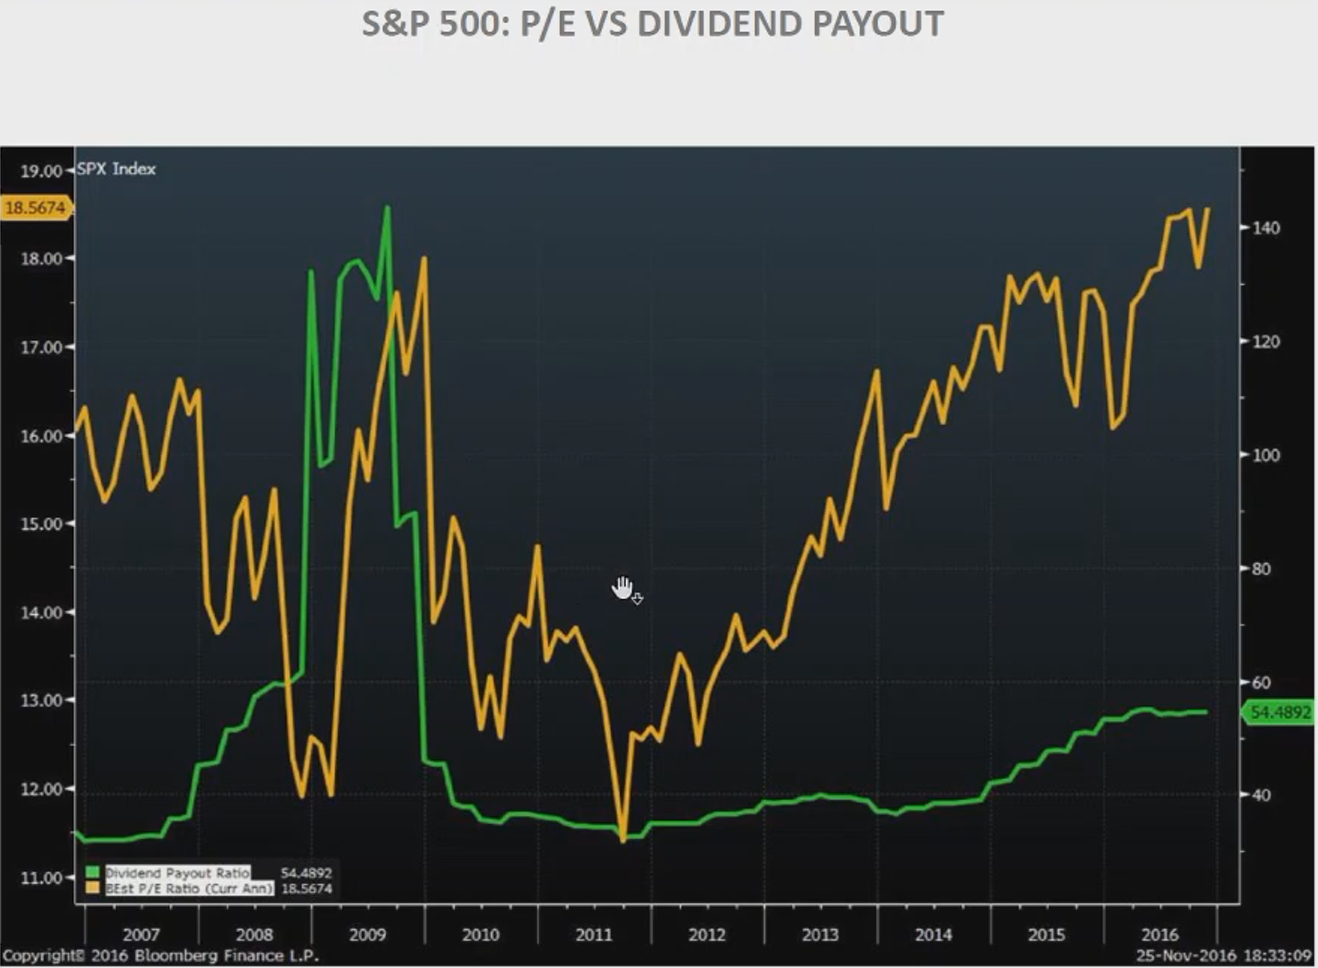
\includegraphics[width=0.75\textwidth]{P_E.png}\\
{жёлтым P/E для S&P 500, зелёным Dividend Payout ratio для S&P 500}
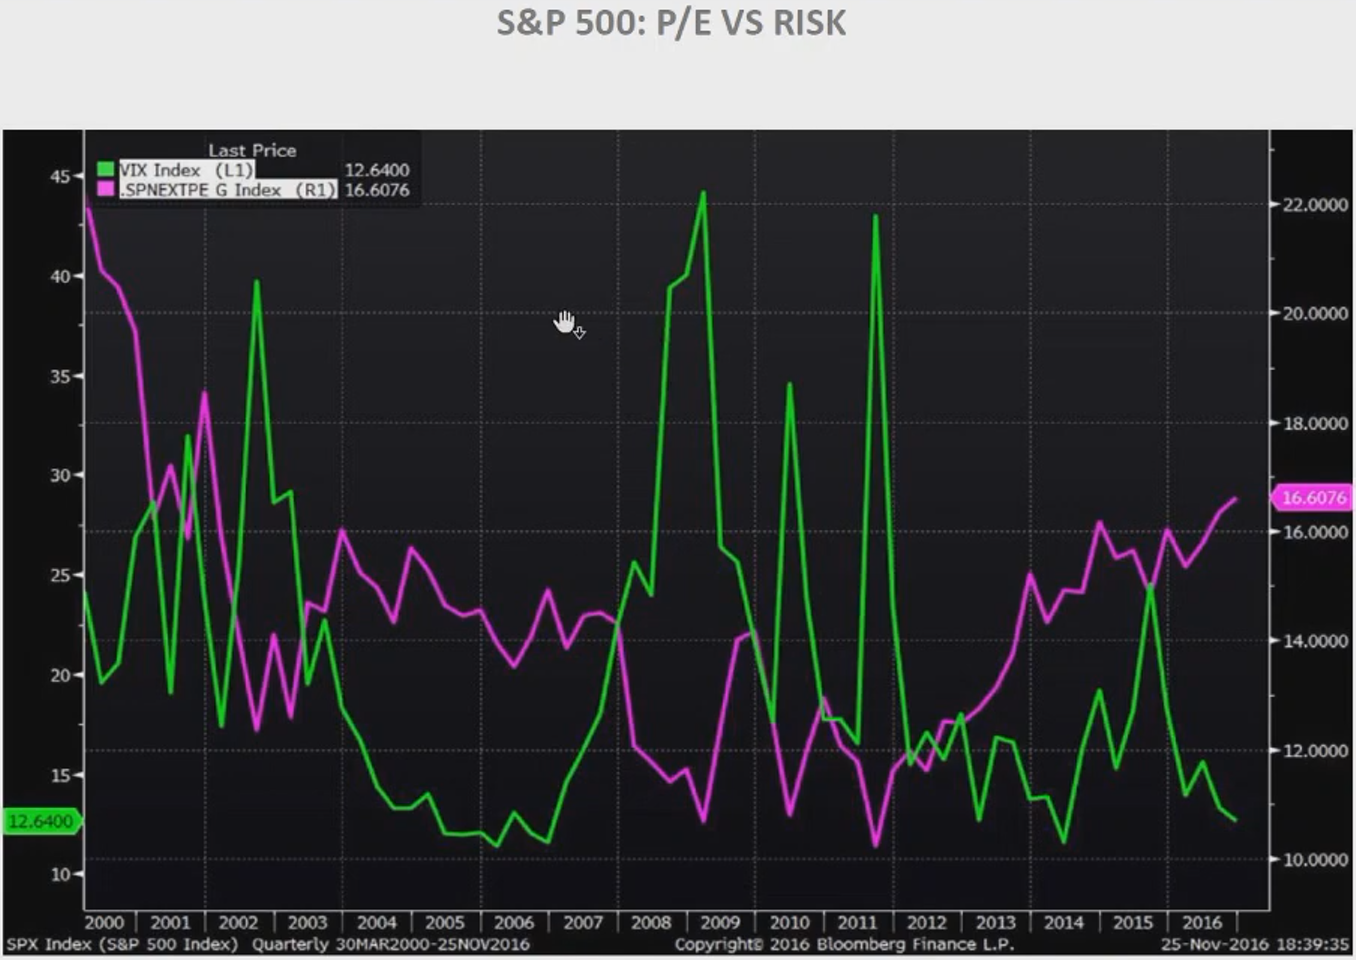
\includegraphics[width=0.75\textwidth]{P_E_2.png}\\
{фиолетовым P/E для S&P 500, зелёным индекс риска(VIX) для S&P 500}\\
\bigskip
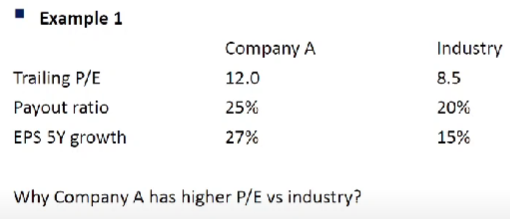
\includegraphics[width=0.75\textwidth]{Example_1.png}\\
\end{center}
\newpage
\section{С чем можно сравнить компанию}
Time series analysis - сравнение с прошлыми или средними значениями для этой же компании\\
Cross-sectional analysis - сравнение с benchmark(эталоном) или с компанией из группой сравнимых\\
\begin{center}
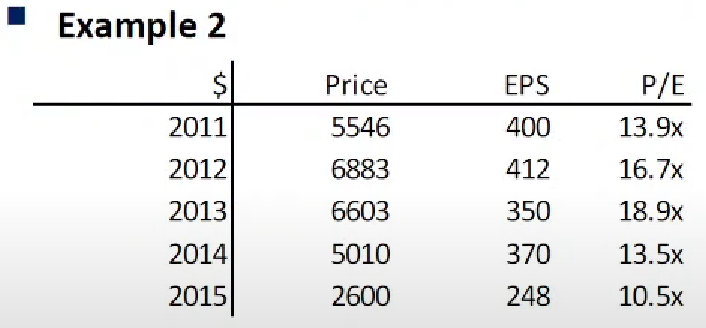
\includegraphics[width=0.75\textwidth]{Example_2.png}\\
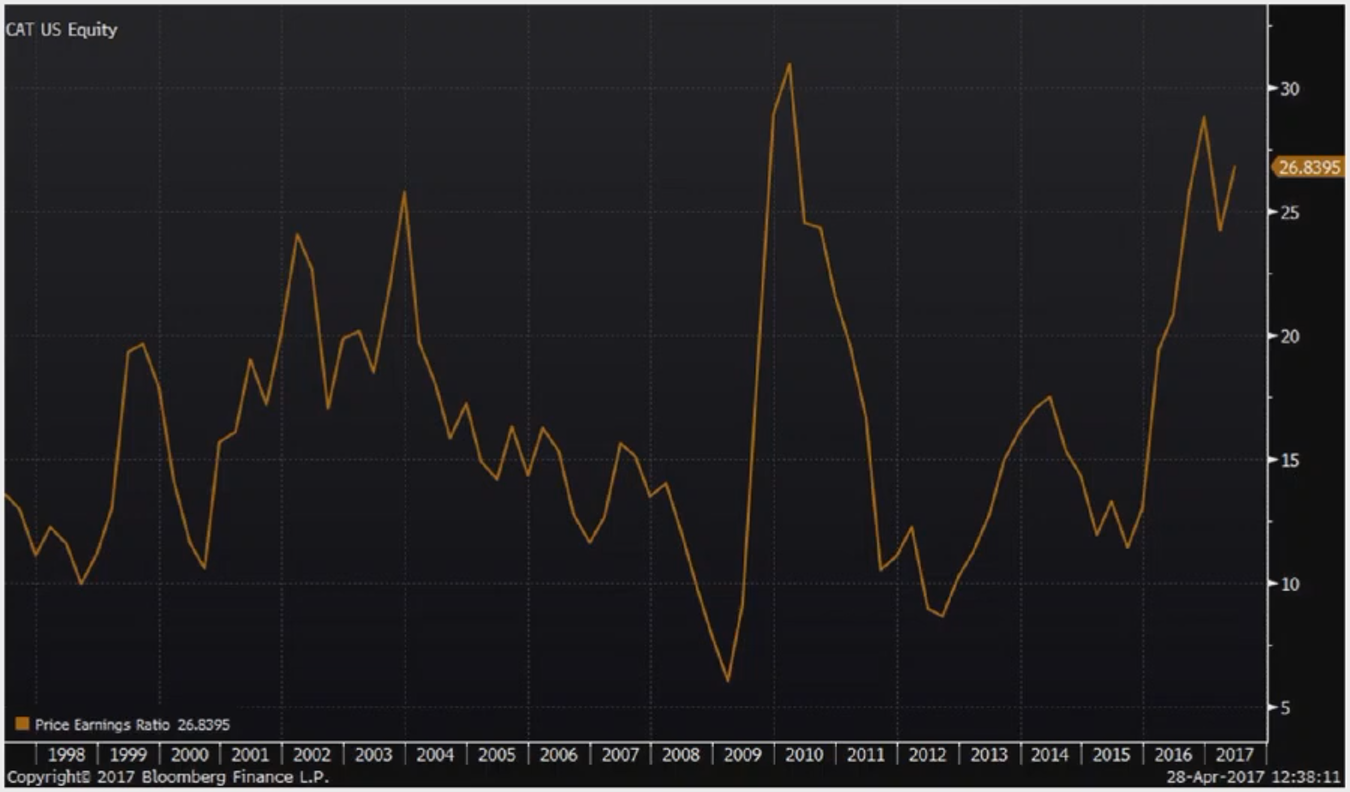
\includegraphics[width=0.75\textwidth]{Hisorical.png}\\
{P/E для акции CATERPILLAR}\
\end{center}
Если компании из одной группы сравнимых, то они должны быть:
\begin{itemize}
    \item В одной индустрии
    \item Одинаковыми по размеру
    \item Из одного географического региона
    \item Сравнимы по темпу роста
    \item Сравнимы по показателю маржинальности
\end{itemize}
\begin{center}
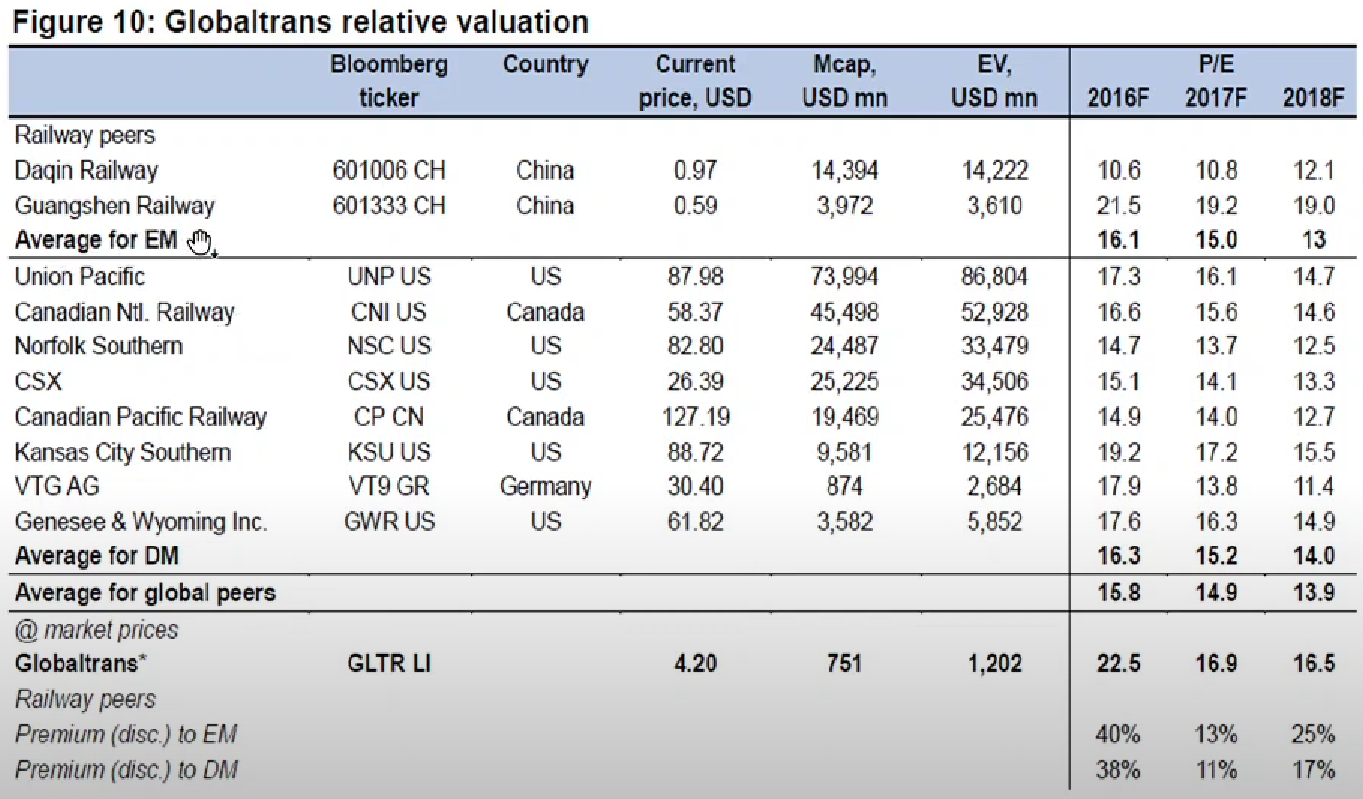
\includegraphics[width=0.75\textwidth]{Relative_valuation.png}\\
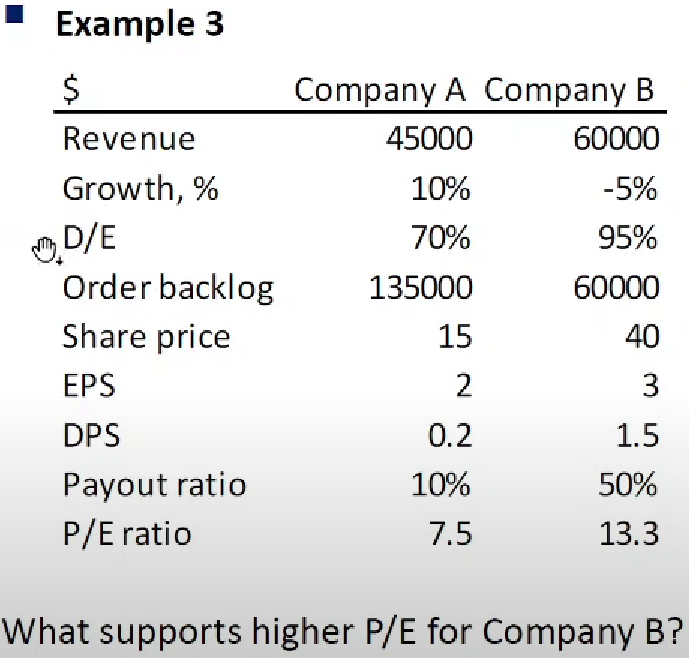
\includegraphics[width=0.55\textwidth]{Example_3.png}\\
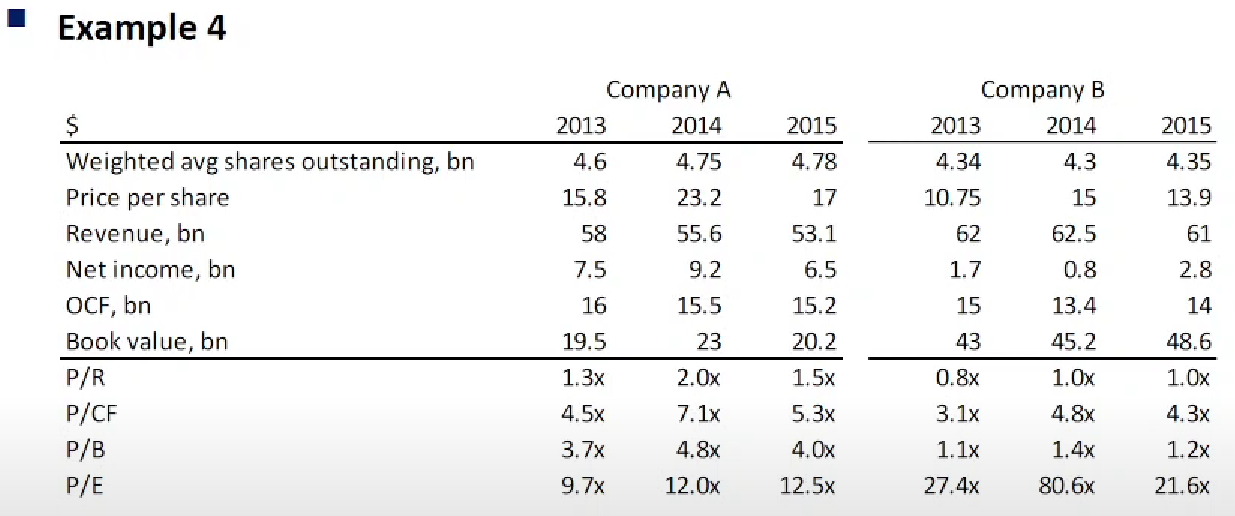
\includegraphics[width=0.75\textwidth]{Example_4.png}\\
\end{center}
\section{Модель мультипликаторов полной стоимости}
EV(enterprise value) Мультипликатор имеет вид Полная стоимость компании(Enterprise value)/финансовый показатель\\
EV = $M_{cap}$ + Debt - Cash and cash equivalents \\
оценка стоимости обыкновенных акций может быть рассчитана косвенно на основе мультипликатора EV.
  Стоимость обязательств и привилегированных акций может быть вычтена из EV, чтобы получить стоимость обыкновенного капитала\\
  Примеры EV Мультипликаторов EV /Revunue, EV/EBITDA, EV/EBIT, EV/FCF.\\
  (Revenue - выручка, EBITDA - прибыль до затрат на налоги на выплату процентов и вычеты по амортизации, EBIT -  прибыль до вычета процентов и налогов, FCF - денежный поток)\\
  Пример:EBITDA=2000, EV/EBITDA=5, Cash=500, Debt=5000, 200 акций в обращении(Number of shares). Хотим узнать цену одной акции(Share price)\\
  EV = EV/EBIDTDA * EBITDA = 5*2000 = 10000.\\
  $M_{cap}$ = EV - Debt + Cash = 10000 - 5000+500 = 5500\\
  Share price = $M_{cap}$/Number of share = 5500/200 = 27,5\\
\begin{center}
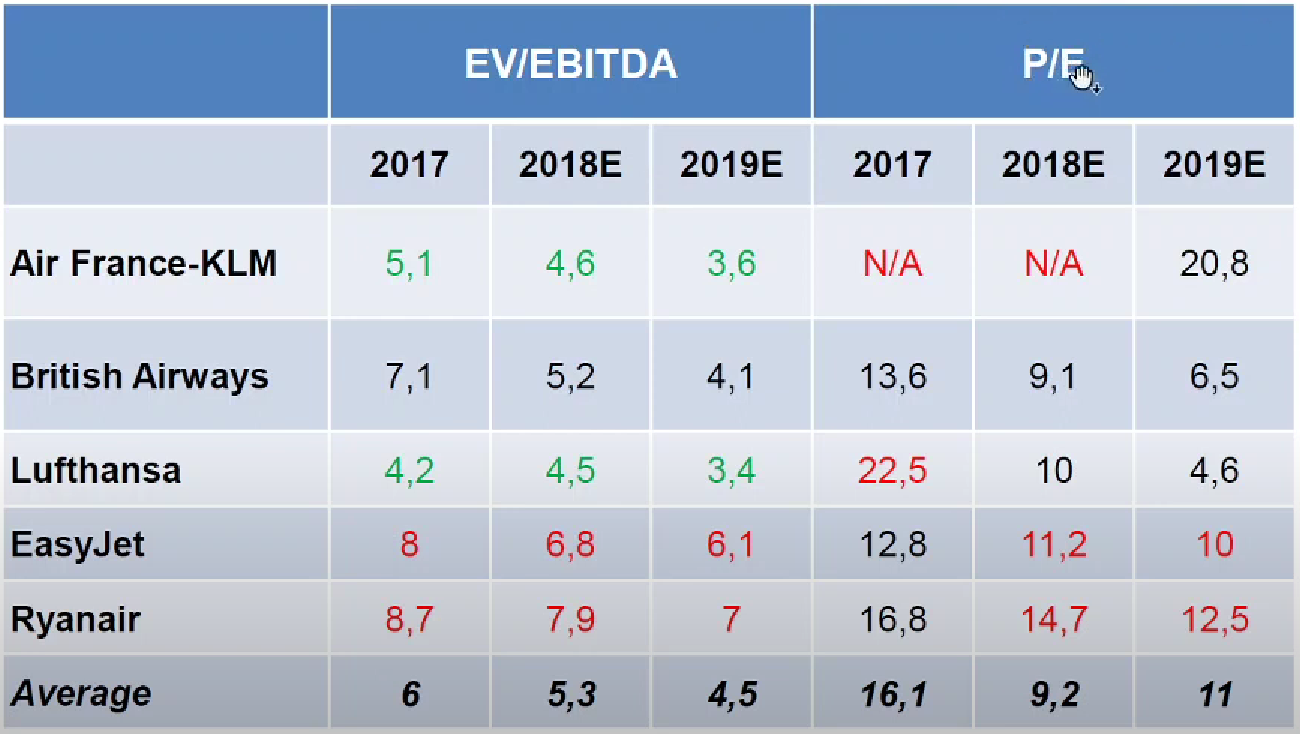
\includegraphics[width=0.75\textwidth]{EV_multiple.png}\\
\end{center}
\newpage
\section{Модели основанные на оценке активов}
Теоретическое обоснование этой группы методов состоит в том что каждая компания публикует финансовую отчетность, соответственно мы можем взять рыночную оценку активов компании, взять рыночную оценку обязательность и таким образом выйти на рыночную оценку с самих акций компании.\\
Оценка на основе активов оценивает рыночную или справедливую стоимость активов и обязательств компании.
Оценки на основе активов хорошо работают для компаний, которые не имеют высокой доли нематериальных активов и имеют высокую долю текущих активов и текущих обязательств.\\
Вычисление оценки на основе активов:\\
\begin{itemize}
    \item Начать с балансовой стоимости активов и обязательств
    \item Процесс оценки
    \item MV активов и обязательств
    \item MV собственного капитала = MV активов - MV обязательств
\end{itemize}

% asset-based valuation is estimating the market or fair value of the company-' assets and liabilities
% asset-based valuations work well for companies that do not have a high proportion of intangible and that do have a high proportion of current assets and current liabilities
%start with book value of assets and liabilities|estimation process|MV of assets and liabilities|MV of equity = MV of assets - MV of liabilities
Проблемы Оценки рыночных активов и обязательств:
\begin{itemize}
    \item Трудно определить MV
    \item BV значительно отличается от MV
    \item У компании много не материальных активов
    \item Быстро растущая инфляция.
\end{itemize}
Оценка стоимости активов против DCF на примере Авиакомпании попавшей в кризис.\\

1) DCF - нет вводных данных для компании\\
2) Оценка стоимости активов - можем оценить соглашения о полётах, договорённости с аэропортами, самолёты имеющиеся в собственности.

\section{Какой метод лучше?}
Методы приведённой стоимости:\\
 Основывается на теории о том что справедливая стоимость акции должно быть равна сумме всех будущих денежных потоков приведенных настоящему моменту\\
 Плюс состоит в том что можно получить именно точную оценку справедливой стоимости \\
 Минус в том что меняя вводные данные в этих наших формулах мы можем получать очень сильно расходящееся результаты\\
Относительная оценка(мультипликаторы):\\
Очень просто посчитать\\
Сложность состоит в том что чтобы действительно сделать правильный вывод нужно сравнивать сравнимые компании(действительно подходящие между собой)\\
Модели оценки активов:\\
в соответствии с представлением о том, что бизнес стоит суммы его частей\\
Сейчас существует не так много подходящих под эту оценку бизнесов из-за сложности с определением рыночной стоимости и стоимости нематериальных активов.


\end{document}
